\documentclass[14pt,a4paper,oneside]{article}

\usepackage[utf8]{inputenc}   


\usepackage{amsmath,amsthm,amssymb,appendix,bm,mathrsfs,ctex,geometry,tcolorbox,fancyhdr,tikz,esint,appendix}


%% GB/T 7714 宏包 ---- 引文格式
\usepackage[sort&compress]{gbt7714}
\bibliographystyle{gbt7714-numerical}



% \numberwithin{equation}{section}             %%%%%% 公式编号




\geometry{left=1.7cm, right=1.7cm, top=2.54cm, bottom=2.54cm}    %%%%% 页面尺寸
\linespread{1.5}                             %%%%% 行距1.5倍
\pagestyle{fancy}



%%    设置页眉页脚
\fancyhf{}
\renewcommand{\headrulewidth}{0.15mm}
\fancyhead[C]{文献阅读报告}                   %%%%%% 页眉
\fancyfoot[C]{\thepage}                      %%%%%% 页脚 页码
\setlength{\headheight}{15pt}


%%   设置各种链接颜色为黑色
\usepackage[colorlinks,
            linkcolor=black,
            anchorcolor=black,
            citecolor=black,
            urlcolor=blue
            ]{hyperref}



%%   例子编号
\newcounter{example}
\counterwithin{example}{subsection}
\newcommand{\examplename}{Example}
\newcommand{\exampleTitle}[1]{%
\textbf{\refstepcounter{example}\examplename\theexample:#1}\par}


%%  插入图片配置
\usepackage{graphicx,subfigure}
\usepackage[]{caption2} %新增调用的宏包
% \numberwithin{figure}{section}               %%%%%% 图片编号按节

\graphicspath{ {./Figure/} }            %%%%% 设置图片文件所在目录
\DeclareGraphicsExtensions{.pdf,.svg,.jpeg,.png,.jpg}     %%%%% 支持图片格式


%%    支持tikz作图
\usepackage{tikz}
\usetikzlibrary{backgrounds,arrows}


\usepackage{pgfplots}
\pgfplotsset{compat=1.15}
\usepackage{mathrsfs}


\title{\textbf{文献阅读报告 11\\Band-edge mediated frequency down-conversion in a gas-filled anti-resonant hollow-core fiber\cite{gavaraBandedgeMediatedFrequency2020}}}                           %%%%% 标题
\author{骆禹天}                                           %%%%% 作者
\date{2024/**/**}                                        %%%%%% 日期

%%   定义一些数学格式
\newtheorem{theorem}{定理}[]
\newtheorem{definition}[theorem]{定义}
\newtheorem{lemma}[theorem]{引理}
\newtheorem{corollary}[theorem]{推论}
\newtheorem{example}[theorem]{例}
\newtheorem{proposition}[theorem]{命题}
\renewcommand{\abstractname}{\Large\textbf{摘要}}




%------------------------- 开始文档  -------------------------%



\begin{document}

\pagenumbering{Roman}         %%%%% 目录前页码统计按罗马数字

\maketitle

\setcounter{page}{1}          %%%%% 标题开始统计页数

%------------------------- 目录  ------------------------------%

\tableofcontents              %%%%% 插入目录

\newpage
\setcounter{page}{1}          %%%%% 目录后重新统计页数


\pagenumbering{arabic}        %%%%% 目录后统计页码为阿拉伯数字



%%%%%%%%%%%%%%%%%%%% 开始第一节  %%%%%%%%%%%%%%%%%%%%%


\section{Introduction}

反谐振空心光纤 (AR-HCF) 优势:

· 宽工作光谱范围: 深紫外-中红外\cite{xiePhotonicsMeetsTopology2018, yuAttenuationLimitSilicabased2019};

· 可承受高平均功率和峰值功率\cite{debordMultimeterFiberdeliveryPulse2014};

· 固有的小波导色散使光学特性可通过改变填充气体种类和压力调节\cite{xuUltraslowWeaklightSolitons2017};

· 特别是, 能在较宽光谱范围内灵活改变色散范围与不同波长激光器配对.

在非线性光学领域有广泛应用:

· 脉冲压缩\cite{xuUltraslowWeaklightSolitons2017};

· 超连续谱生成\cite{jacobsonGlobalAreasLow2019};

· 非线性频率转换\cite{belliHighlyEfficientDeep2019}.

作者特别注意到 AR-HCF 在近红外到紫外中的孤子泵浦转换的众多演示\cite{jolyBrightSpatiallyCoherent2011a, kottigModulationalinstabilityfreePulseCompression2020, cimekSynthesisConditionsZBLAN2018}. 这是因为 AR-HCF 中波导色散分布紧密遵循 Marcatili 和 Schmeltzer 模型\cite{marcatiliHollowMetallicDielectric1964a}, 有利于在较短波长中进行孤子相位匹配. 另一方面, 相同的理念不能直接应用于转换到更长的波长, 因为该模型不支持在红色侧进行相位匹配. 

迄今已提出一些技术实现近红外飞秒脉冲转换为较SPM更长的波长. 

· 光电离介导短时折射率变化, 以暂时在中红外区域实现相位匹配\cite{kottigMidinfraredDispersiveWave2017, novoaPhotoionizationinducedEmissionTunable2015}. 

· 级联四波混频驱动正常色散状态下 1 $\mathrm{\mu m}$ 处泵浦转换为 3-4 $\mathrm{\mu m}$ 的辐射\cite{hasanMidinfraredPulseGeneration2019}. 

AR-HCF 纤芯-包层界面处薄介电壁的存在引入了一系列高损耗共振带, 谐振位置由壁厚决定. 传输带位于这些谐振带之间. 结构共振对非线性脉冲传播的影响是一个积极研究的主题\cite{qiEssentialsResonanceenhancedSolitonbased2020, wuImpactNonlinearEffects2020}. 考虑这些谐振时的一个显着特征是传输带边缘附近色散的快速变化, 这与 Marcatili 和 Schmeltzer 模型控制的中心部分的色散无关. 利用充气 AR-HCF 中的带边效应的想法已被用于增加超连续谱生成中的输出带宽\cite{sollapurResonanceenhancedMultioctaveSupercontinuum2017}. 在另一项工作中, 这种效应在泵浦传输带的蓝色边缘带来的孤子相位匹配导致了较短波长内的强窄带辐射\cite{changInfluenceIonizationUltrafast2011a}. 

本文作者利用 AR-HCF 中的带边效应来演示近红外泵浦到更长波长的相位匹配转换. 在 800 nm 的第二个传输带中泵浦, 并在 1.45 $\mathrm{\mu m}$ 左右产生辐射, 该辐射位于第一个传输带的蓝色边缘. 这种方法产生辐射波长仅取决于反谐振包层管的壁厚. 其他参数如气压和泵浦能量, 虽仍与在初始阶段引起足够光谱展宽有关, 但并不决定输出波长. 

\section{Set-up}

\begin{figure}[h]
    \centering
    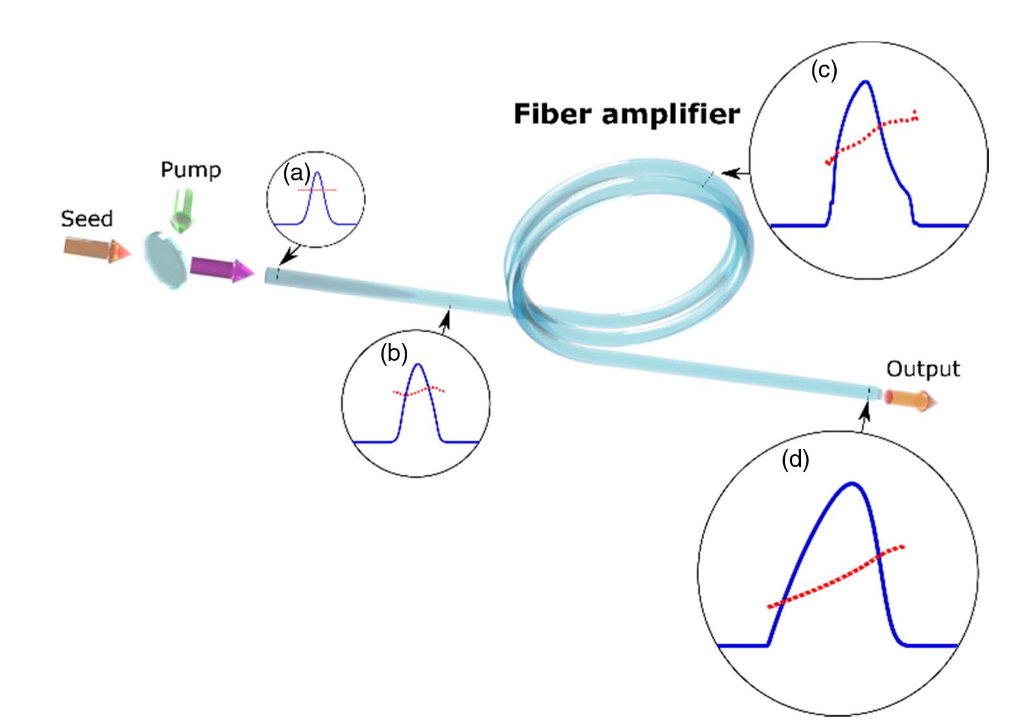
\includegraphics[width=0.5\textwidth]{p1.png}
    \caption{实验装置: M1和M2, 转向镜； L1, 输入耦合透镜； L2, 输出准直透镜； C1,C2, 气室. }\label{p1}
\end{figure}

· AR-HCF, 光纤末端放置于两气室中通过氩气加压, 一端飞秒激光泵浦, 另一端输出;

· 气室窗口提供光学通道. C1 窗口: 在泵浦处具有抗反射涂层的石英玻璃, C2: 窗口是无涂层蓝宝石玻璃. 输入和输出窗口损耗分别约为 1\% 和 8\%. 

· 泵浦激光: 800 nm, 40 fs,  1 kHz. 

· 用消色差模式匹配透镜 L1 将光束耦合到系统中, 并用准直透镜 L2 收集输出. 

\begin{figure}[h]
    \centering
    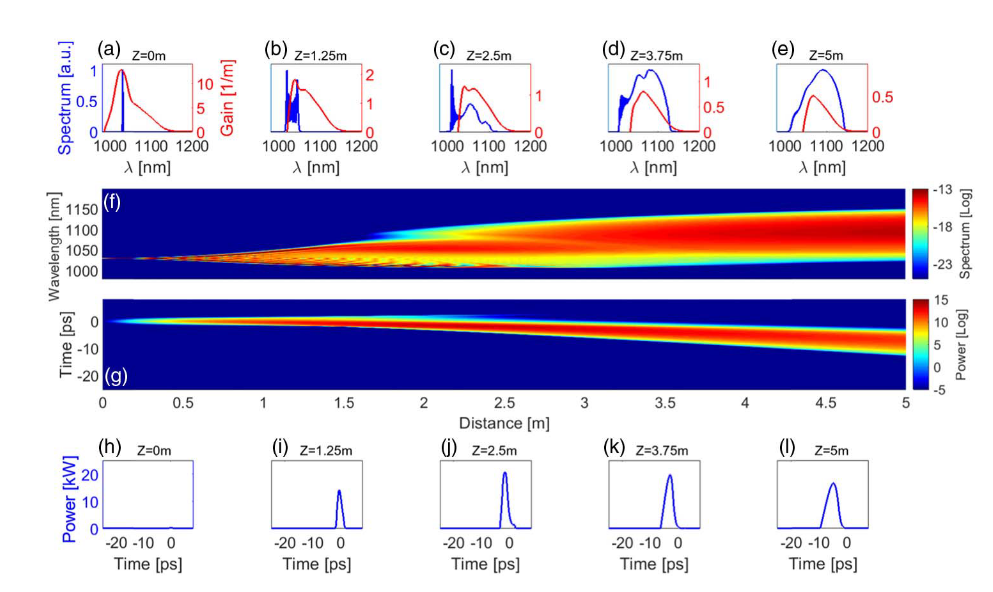
\includegraphics[width=0.5\textwidth]{p2.png}
    \caption{(a) AR-HCF 截面扫描电子显微照片.  (b) 管壁放大图.  (c) 800 nm 泵浦输出光束模式轮廓.  (d) 使用削减法测量 AR-HCF 传输损耗,  TB1, TB2 和 RB1, RB2 分别是前两个传输带和谐振带. }\label{p2}
\end{figure}

· AR-HCF 纤芯直径 30 $\mathrm{\mu m}$. 包层管间间隙 6-10 $\mathrm{\mu m}$, 管壁厚600 ($\pm 50$) nm [图\ref{p2}].

· 800 nm 泵浦输出光束轮廓如图 \ref{p2}(c) 所示, 类高斯空间分布表明大部分耦合光处于基模. 

图 2(d) : 基于超连续谱源通过削减法测量的 AR-HCF 在 0.4-1.7 $\mathrm{\mu m}$ 传输损耗. 

· 第一传输带 (TB1): 1.4 $\mathrm{\mu m}$ 左右-红外区域. 

· 第二传输带 (TB2): 0.7-1 $\mathrm{\mu m}$. 

· 两者间存在第一谐振带(RB1) .  

· 800 nm 泵浦落在 TB2 内, 此频段损耗 $<0.3 \;\mathrm{dB\; m^{-1}}$, 相对实验的长度尺度足够低. 

· 作者使用 75 cm 长 AR-HCF, TB1 蓝色边缘在 1.45 $\mathrm{\mu m}$ 损耗为 $\sim3 \;\mathrm{dB \;m^{-1}}$.  

· 0.6 $\mathrm{\mu m}$ 以下谐振带较多, 后续谐振带间间距随波长减小而减小. 然而对它们的表征受到超连续谱源亮度缺乏限制. 

\section{光谱测量}

\begin{figure}[h]
    \centering
    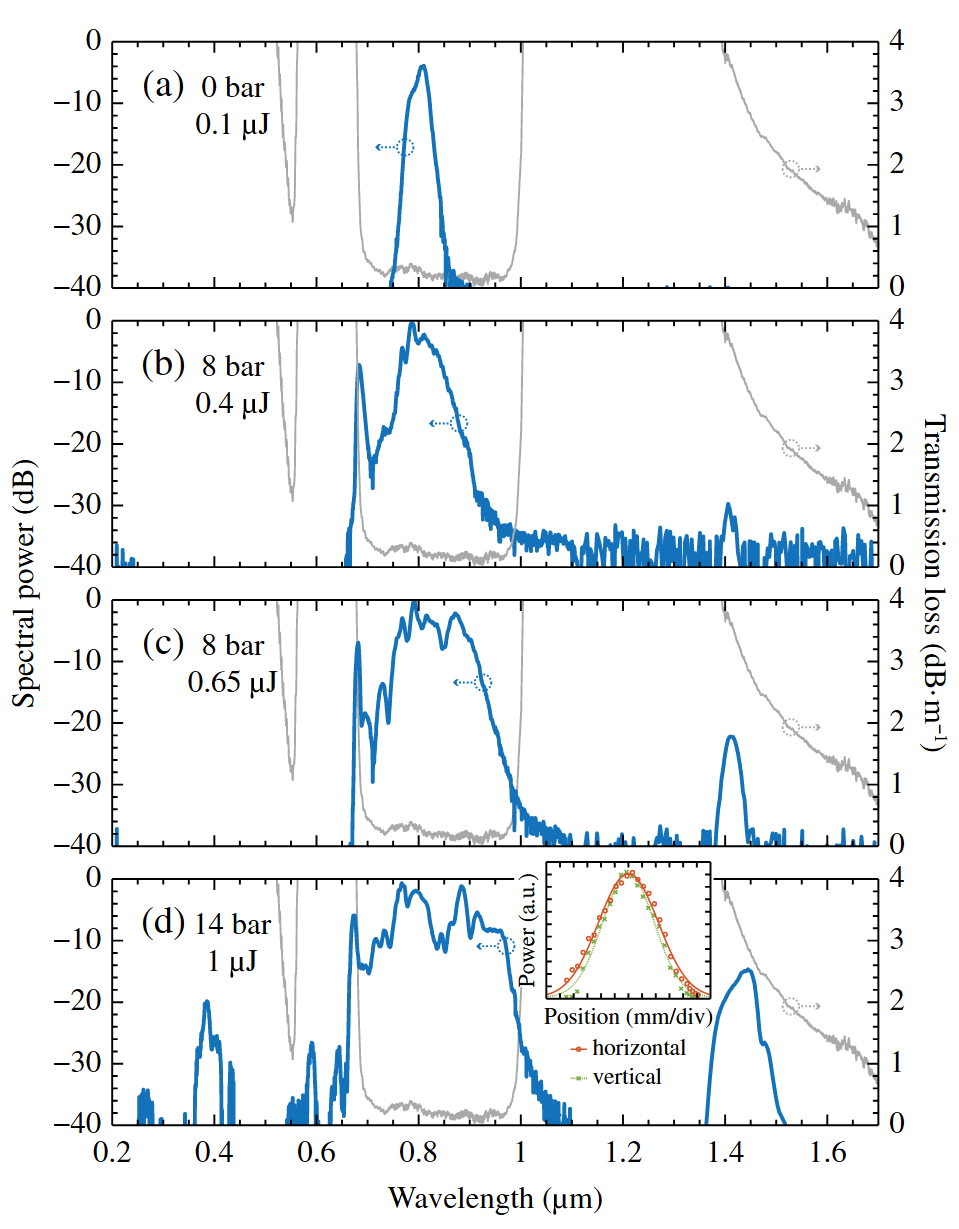
\includegraphics[width=0.5\textwidth]{p3.png}
    \caption{不同氩气压力和泵浦能量下, 75 cm AR-HCF 输出光谱.  (a) 0 bar, 0.1 $\mathrm{\mu J}$ (b) 8 bar, 0.4 $\mathrm{\mu J}$ (c) 8 bar, 0.65 $\mathrm{\mu J}$.  (d) 14 bar, 1 $\mathrm{\mu J}$. 插图: 使用刀口技术获得的 1.45 $\mathrm{\mu m}$ 波段输出光束轮廓. 灰线: 0.4-1.7 $\mathrm{\mu m}$ 范围内的光纤损耗}\label{p3}
\end{figure}

图 \ref{p3} 不同氩气压力和泵浦能量下输出光谱, 结果分析:

· 随泵浦能量和气压增加, 光谱通过自相位调制变宽. 

· 随非线性持续增加, 开始在 1.45 $\mathrm{\mu m}$ 左右观察到强发射带, 位于 AR-HCF 第一传输频带的蓝色边缘附近, 而泵浦位于第二传输频带中. 

· 由后续, 这种强发射归因于到带边缘的两个单独的相位匹配转换, 一个以色散波 (DW) 生成的形式, 另一个通过简并四波混频 (DFWM) 的形式. 

· 改变泵浦能量或气体压力, 发射波长也不变 [图 \ref{p3}]. 相反, 它由谐振带的位置决定, 而谐振带位置由介电壁厚度决定. 

· 在图\ref{p3} (d) 中, 1.45 $\mathrm{\mu m}$ 发射很强, 仅比泵浦强度低约一个量级. 该频段来自基模 [插图], 能量占总输出 2.2\%. 

· 短波一侧, 注意到另一个峰值, 其强度随着 0.68 $\mathrm{\mu m}$ 处非线性增加而增加. 这是 AR-HCF 第二传输带的蓝色边缘, 由于该区域色散的急剧变化而出现向该波长的转换. 

· 0.6 $\mathrm{\mu m}$ 以下出现几个低强度峰, 其中在 0.4 $\mathrm{\mu m}$ 处有一个显着峰. 在这里, 许多包层壁厚引起的高阶谐振带看起来间隔很近, 因此色散主要由谐振决定. 这可以产生多个相位匹配点. 

\section{数值分析}

基于单向场传播方程\cite{changInfluenceIonizationUltrafast2011b}
\begin{equation}
    \partial_z\mathbf{E}(z,\omega)=i\left(\beta-\frac\omega v+i\frac\alpha2\right)\mathbf{E}(z,\omega)+i\frac{\omega^2}{2c^2\beta}\mathcal{F}\{\chi^{(3)}\mathbf{E}(z,t)^3\}
    \label{eq:1}
\end{equation}
其中, 

· 仅考虑 $\mathrm{HE_{11}}$ 模传播, 忽略其与高阶模式相互作用. 

· 色散用 $\beta$ 表示, 压力相关气体贡献来自 Sellmeier 方程, 波导贡献及有效模式面积使用经验公式\cite{hasanEmpiricalFormulaeDispersion2018}计算. 

· 作者发现传输带中模式面积色散相对较小\cite{gavaraBandedgeMediatedFrequency2020a}, 因此忽略.  

· AR-HCF 的衰减采用测量的损耗 [图 \ref{p2} (d)].

· 注意, 假设色散采用理想光纤结构, 而实际测量传输损耗的光纤几何形状中可观察到一些不均匀性, 导致模拟使用损耗和色散存在一些差异, 特别是在谐振带紧密堆积的 0.6 $\mathrm{\mu m}$ 以下. 然而, 其影响在主要特征出现的前两个传输和谐振频带中可忽略不计.  

· $\chi^{(3)}$ 是加压氩气的三阶磁化率\cite{lehmeierNonresonantThirdOrder1985a}. 

图 \ref{p4} (a) 显示了在传播充满 14 bar 氩气的 75 厘米长 AR-HCF 后, 以 800 nm 为中心、FWHM 持续时间为 40 fs 的 1 $\mathrm{\mu J}$ 泵的模拟输出光谱. 测量的光谱一起呈现, 以便以灰色阴影进行比较. 与 1.45 和 0.68 $\mathrm{\mu m}$ 附近的辐射细节吻合良好, 这在模型中得到了很好的反映. 我们强调, 在我们的数值模拟中, 这些辐射的位置不会随着泵浦脉冲能量或气体压力的变化而改变——这证明它们是由带边效应引起的. 光谱演变绘制在图 \ref{p4} (b) 的伪彩色图中. 最初, 泵浦在反常色散区域中经历自相位调制引起的光谱展宽, 最终主光谱的尾部到达图4中垂直虚线所示的带边缘中的相位匹配点. 

\begin{figure}[h]
    \centering
    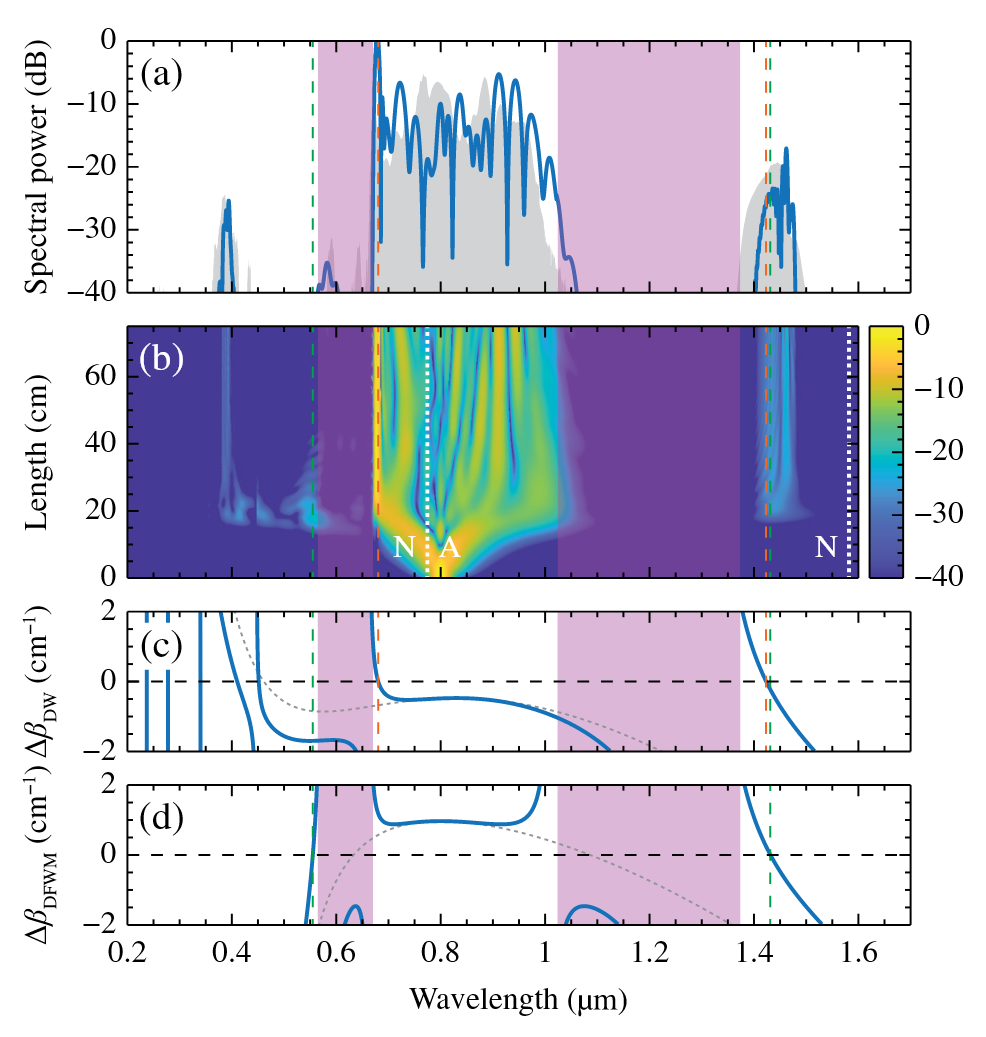
\includegraphics[width=0.5\textwidth]{p4.png}
    \caption{(a)模拟输出光谱, 灰色阴影: 相同条件实验测量光谱 (b) 光谱沿光纤演变, 前两个传输带零色散波长用白色虚线标记, N, A : 正常, 反常色散区域 (c) 800 nm 孤子的 DW 相位匹配图, 红色虚线表示 DW 的两个相位匹配点 (d) 800 nm 泵浦的 DFWM 相位匹配图, 绿色虚线标记相位匹配的信号/闲频波长.  (c) 和 (d) 中的灰色虚线是模型中不考虑谐振时的相位失配. 洋红色调是前两个共振带. }\label{p4}
\end{figure}

有两种独特的混频过程负责这些相位匹配. 

第一个是 DW 生成\cite{carlsonPhotonicchipSupercontinuumTailored2017}. 其相位匹配的计算公式为
\begin{equation}
    \Delta\beta_{\mathrm{DW}}=\beta-\beta_0-\beta_1(\omega-\omega_0)-\Gamma 
    \label{eq:2}
\end{equation}
其中, $\beta_n$ 是泵浦 $\omega_0$ 处 $\beta$ 的第 n 个泰勒级数展开系数, $\Gamma=\frac38\frac{\omega^2}{c^2\beta}\chi^{(3)}|E_0|^2$ 是峰值输入场强 $E_0$ 的非线性校正项. 

· 如图 \ref{p4} (c) 所示, 相位匹配波长用红色虚线标记. 靠近谐振处强的色散有利于在每个传输带蓝色端的零相位失配. 在实验和模拟中都发现了 0.4 $\mathrm{\mu m}$ 处的峰值, 归因于相位匹配, 如图 \ref{p4} (c) 所示. 

负责频率下变频到 1.45 $\mathrm{\mu m}$ 频段的第二种机制是 DFWM\cite{andersen7thEuropeanConference1975}. 它必须满足光子能量和动量守恒：
\begin{equation}
    2\omega_p=\omega_s+\omega_i,\quad2\beta_p=\beta_s+\beta_i+2\Gamma_p
    \label{eq:3}
\end{equation}
其中 $\omega_p$ 、 $\omega_s$ 和 $\omega_i$ 分别是泵浦光、信号光和闲频光的角频率,  $\beta_p$ 、 $\beta_s$ 和 $\beta_i$ 是相应的波矢量,  $\Gamma_p$ 是由泵浦估计的非线性校正项. 相位失配 $\Delta \beta_ {\mathrm{DFWM}}$ 满足方程 (\ref{eq:3}).

· 泵浦波长为 800 nm, 如图 \ref{p4} (d) 所示. 两条绿色虚线是相位匹配的信号/闲频信号, 并且谐振决定了它们的位置. 其中之一的波长 1.43 $\mathrm{\mu m}$, 对长波长的发射带有额外的贡献. 

· 另一方面, 0.56 $\mathrm{\mu m}$ 频率上转换光子由于高损耗而很快丢失. 

在这两个过程中, 包层壁厚引起的谐振的存在对于实现长波长的相位匹配至关重要. 它们对色散的影响主导并推翻了 Marcatili 和 Schmeltzer 模型所设定的影响, 使得在附近产生辐射成为可能. 

\begin{figure}[h]
    \centering
    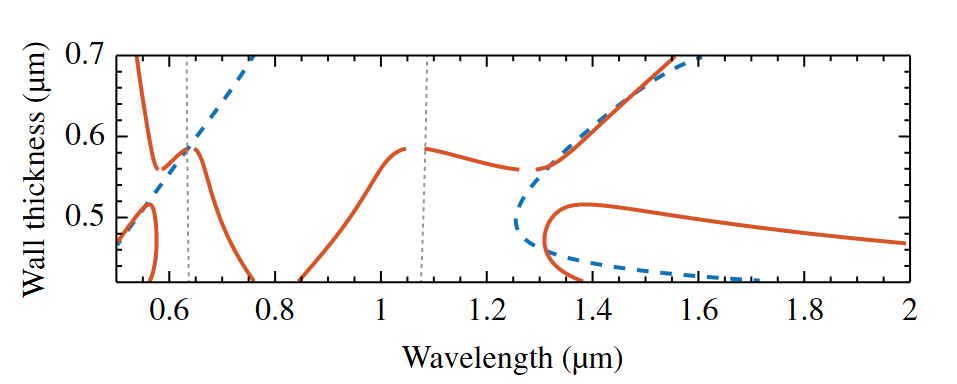
\includegraphics[width=0.5\textwidth]{p5.png}
    \caption{包层壁厚与 DW (蓝色虚线) 和 DFWM (红色实线, 信号/闲频信号在 0.5-2 $\mathrm{\mu m}$ 内, 泵浦波长为 800 nm) 相位匹配点. 灰色虚线是色散模型中没有共振时的相位匹配. }\label{p5}
\end{figure}

图 \ref{p5} 分别以蓝色虚线和红色实线显示了针对不同壁厚计算的 DW 和 DFWM 相位匹配点. 这里考虑的壁厚范围将 800 nm 泵浦置于第二传输波段. 两条灰色虚线表示色散模型中没有共振时的相位匹配, 突出显示了它们在相位匹配图中的作用. 


%--------------------  插入参考文献  --------------------%

\newpage

\clearpage           %%%  “目录”中显示的页码正确, 需要添加 \clearpage
\phantomsection      %%   “目录”中的链接能正确跳转, 需要添加 \phantomsection
\addcontentsline{toc}{section}{参考文献}   %向目录中添加条目, 以章的名义

\bibliography{ref}

\end{document}